% Aleja y Mariana:
% Aqui esta la presentacion de openCv, ya estan todos los temas en
% la tabla de contenidos, la idea de esto es que podamos aprender
% de openCv y latex al tiempo.
%
% Para poder terminar la presentacion se necesitan varias cosas
%
%     1) Agreguen su nombre a los autores (reemplacen en donde dice !nombres!)
%     2) Explicar cada una de las partes de OpenCv (son 8)
%     3) El codigo de todos los ejemplos ya esta listo, pero necesito
%        que por favor expliquen cada uno.
%     4) Para la seccion de thresholding se necesita un poco mas de informacion
%        por favor llenar las diapositivas explicando que es la manipulacion
%        de pixeles y como se hace thresholding en cada caso
%
% Si quieren ver los ejemplos funcionando al final del pdf esta la explicacion.
%
% Para que les sea mas facil buscar la informacion en drive esta el libro en
% el que me base para hacer los ejemplos. Se llama Instant openCv started,
% pero el archivo se llama OpenCv1.pdf, esta en la carpeta 2016/Libros
%
% Con ese libro tienen para sacar toda la informacion
%
% Muchas gracias

\documentclass{beamer}

\usepackage{listings}

\begin{document}

    \title{OpenCv Kata}
    \author{!nombres! \\
            Alejandro Salgado G}
    \date{6 de Febrero de 2016}

    \frame{ \titlepage }

    \frame{
    \frametitle{Tabla de contenidos}

    \begin{enumerate}
        \item Diferencia entre Git y GitHub
 	    \item Servidores de repositorios Git
        \item Instalar Git
        \item C\'omo crear un repositorio?
	   \item Los tres estados

	  %\item Principales conceptos
        \item C\'omo compartir un repositorio?
        \item Committing, Pull y Push
        \item C\'omo crear un Brach?
        \item Merging
    \end{enumerate}
}

    \frame{
    \frametitle{Partes de OpenCv}

    OpenCv se divide en 8 partes.

    \begin{figure}
        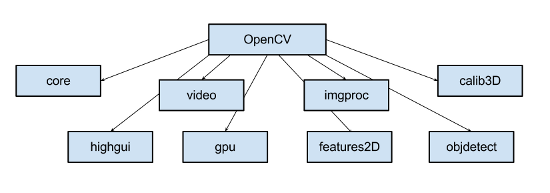
\includegraphics[scale=0.5]{Image/OpenCv}
    \end{figure}

    Imagen tomada de:
    https://www.packtpub.com/sites/default/files/Article-Images/8812\_03\_01.png
}

    \begin{frame}[fragile]
   \frametitle{Leer y mostrar una imagen}

        En este ejemplo se necesitan 2 modulos de OpenCv

        \begin{enumerate}
            \item Core para poder leer la imagen
            \item Highgui para poder mostrarla
        \end{enumerate}

        \vspace{1cm}

        En Codigo se ve asi:

        \lstset{ morecomment=[l][\color{blue}]{\#} }
        \begin{lstlisting}
    #include "opencv2/highgui/highgui.hpp"
    #include "opencv2/core/core.hpp"
        \end{lstlisting}

        Adicionalmente se debe usar el namespace o espacio de nombre de OpenCv:

        \lstset{ morecomment=[l][\color{blue}]{using} }
        \begin{lstlisting}
    using namepace cv;
        \end{lstlisting}
\end{frame}

    \begin{frame}[fragile]
   \frametitle{Leer y mostrar una imagen}

    Por ultimo esta el codigo fuente:

    \scriptsize

    \begin{lstlisting}
int main(int argc, char *argv[]){

    Mat image = imread( /* ruta de la imagen */ );
    namedWindow( "Window", CV_WINDOW_AUTOSIZE );
    imshow( "Window", image );
    waitKey(0);

    return 0;

}
    \end{lstlisting}

\end{frame}

    \begin{frame}[fragile]
   \frametitle{Cambiar medida}

        En este ejemplo se necesitan 3 modulos de OpenCv

        \begin{enumerate}
            \item Core para poder leer la imagen
            \item Highgui para poder mostrarla
            \item Imgproc para poder modificarla
        \end{enumerate}

        \vspace{1cm}

        En Codigo se ve asi:

        \lstset{ morecomment=[l][\color{blue}]{\#} }
        \begin{lstlisting}
    #include "opencv2/highgui/highgui.hpp"
    #include "opencv2/core/core.hpp"
    #include "opencv2/imgproc/imgproc.hpp"
        \end{lstlisting}

        Adicionalmente se debe usar el namespace o espacio de nombre de OpenCv:

        \lstset{ morecomment=[l][\color{blue}]{using} }
        \begin{lstlisting}
    using namepace cv;
        \end{lstlisting}
\end{frame}

    \begin{frame}[fragile]
   \frametitle{Cambiar medida}

    Por ultimo esta el codigo fuente:

    \scriptsize

    \begin{lstlisting}
int main(int argc, char *argv[]){

    Mat original, resized, saved;

    original = imread( /* ruta de la imagen */ );
    namedWindow("Original image", CV_WINDOW_AUTOSIZE );
    imshow("Original image", original );

    resize(original, resized, Size(), 0.5, 0.5, INTER_LINEAR);
    namedWindow("Resized image", CV_WINDOW_AUTOSIZE);
    imshow("Resized image", resized );

    waitKey(0);

    return 0;

}
    \end{lstlisting}

\end{frame}

    \begin{frame}[fragile]
   \frametitle{Guardar imagen}

        Al igual que en el ejemplo anterior aqui se necesitan 3 modulos de OpenCv

        \begin{enumerate}
            \item Core para poder leer la imagen
            \item Highgui para poder mostrarla
            \item Imgproc para poder modificarla
        \end{enumerate}

        \vspace{1cm}

        En Codigo se ve asi:

        \lstset{ morecomment=[l][\color{blue}]{\#} }
        \begin{lstlisting}
    #include "opencv2/highgui/highgui.hpp"
    #include "opencv2/core/core.hpp"
    #include "opencv2/imgproc/imgproc.hpp"
        \end{lstlisting}

        Adicionalmente se debe usar el namespace o espacio de nombre de OpenCv:

        \lstset{ morecomment=[l][\color{blue}]{using} }
        \begin{lstlisting}
    using namepace cv;
        \end{lstlisting}
\end{frame}

    \begin{frame}[fragile]
   \frametitle{Guardar imagen}

    codigo fuente:

    \scriptsize

    \begin{lstlisting}
int main(int argc, char *argv[]){

    Mat original, resized, saved;

    original = imread( /* ruta de la imagen */ );
    namedWindow( "Original image", CV_WINDOW_AUTOSIZE );
    imshow( "Original image", original );

    resize( original, resized, Size(), 0.5, 0.5, INTER_LINEAR );

    imwrite( /* ruta de la imagen */, resized);

    namedWindow( "Image saved", CV_WINDOW_AUTOSIZE);
    saved = imread( /* ruta de la imagen */ );
    imshow("Image saved", saved);

    waitKey(0);

    return 0;
}
    \end{lstlisting}

\end{frame}

    \frame{
   \frametitle{Que es la manipulacion de pixeles?}
   
    Utilizar los elementos que  componen una imagen con el fin de obtener informacion de esta o modificarla para un fin en especifico.


    \begin{figure}
        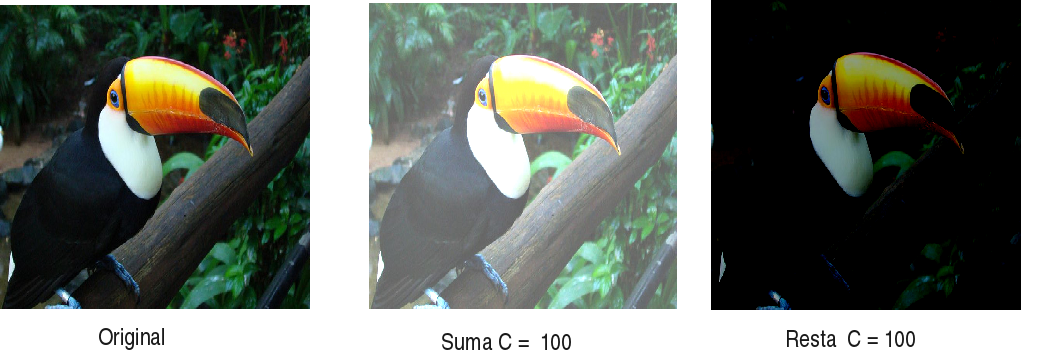
\includegraphics[scale=0.2]{Image/tucan}
    \end{figure}

    Imagen tomada de: 
    https://yetanotherlog.wordpress.com/2011/11/18/log-0-manipulacion-basica-de-imagenes/
}

    \frame{
   \frametitle{Que es Thresholding?}
}

    \frame{
   \frametitle{Como funciona el Thresholding para imagenes a color?}
}

    \frame{
   \frametitle{Como funciona el Thresholding para imagenes grises?}
}

    \begin{frame}[fragile]
   \frametitle{Manipulacion de pixeles (Thresholding)}

        Igual que en el ejemplo anterior se necesitan 3 modulos de OpenCv

        \begin{enumerate}
            \item Core para poder leer la imagen
            \item Highgui para poder mostrarla
            \item Imgproc para poder modificarla
        \end{enumerate}

        \vspace{1cm}

        En Codigo se ve asi:

        \lstset{ morecomment=[l][\color{blue}]{\#} }
        \begin{lstlisting}
    #include "opencv2/highgui/highgui.hpp"
    #include "opencv2/core/core.hpp"
    #include "opencv2/imgproc/imgproc.hpp"
        \end{lstlisting}

        Adicionalmente se debe usar el namespace o espacio de nombre de OpenCv:

        \lstset{ morecomment=[l][\color{blue}]{using} }
        \begin{lstlisting}
    using namepace cv;
        \end{lstlisting}
\end{frame}

    \begin{frame}[fragile]
   \frametitle{Manipulacion de pixeles (Thresholding)}

    Este codigo fuente esta dividido en 4 partes

    \begin{enumerate}
        \item Convertir una imagen de color a escala de grises
        \item Thresholding para color
        \item Thresholding para escala de grises
        \item Main
    \end{enumerate}

\end{frame}

    \begin{frame}[fragile]
   \frametitle{Manipulacion de pixeles (Thresholding)}

   Convertir a gris:

    \scriptsize

    \begin{lstlisting}
Mat convertGray(Mat &color){

    Mat gray; gray.create(color.rows, color.cols, CV_8UC1);
    cvtColor(color, gray, CV_BGR2GRAY);

    namedWindow("Gray image", CV_WINDOW_AUTOSIZE);
    imshow("Gray image", gray);

    return gray;

}

    \end{lstlisting}

\end{frame}

    \begin{frame}[fragile]
   \frametitle{Manipulacion de pixeles (Thresholding)}

   Thresholding para grises:

    \scriptsize

    \begin{lstlisting}
Mat thresholdingGray(Mat &image, uchar thresholdValue){

    for(int i=0; i < image.rows; i++){
        for(int j=0; j<image.cols; j++){

            uchar value = image.at<uchar>(i,j);
            if(value > thresholdValue) image.at<uchar>(i,j)=255;

        }
    }

    return image;
}

    \end{lstlisting}

\end{frame}

    \begin{frame}[fragile]
   \frametitle{Manipulacion de pixeles (Thresholding)}

   Thresholding para color:

    \scriptsize

    \begin{lstlisting}
Mat thresholdingColor(Mat &image, uchar thresholdValue){

    for(int i=0; i < image.rows; i++){
        for(int j=0; j<image.cols; j++){

            int sum = image.at<Vec3b>(i,j)[0] +
                      image.at<Vec3b>(i,j)[1] +
                      image.at<Vec3b>(i,j)[2];

            uchar average = sum/3;

            if(average > thresholdValue){

                image.at<Vec3b>(i,j)[0] = 255;
                image.at<Vec3b>(i,j)[1] = 255;
                image.at<Vec3b>(i,j)[2] = 255;

            }
        }
    }

    return image;
}
    \end{lstlisting}

\end{frame}

    \begin{frame}[fragile]
   \frametitle{Manipulacion de pixeles (Thresholding)}

   Main:

    \tiny

    \begin{lstlisting}
int main(int argc, char *argv[]){

    Mat color = imread( /* ruta de la imagen */ );

    namedWindow("Normal image", CV_WINDOW_AUTOSIZE);
    imshow("Normal image", color);

    Mat gray = convertGray(color);

    Mat colorConverted = thresholdingColor( color, 100 );

    namedWindow("Color image after thresholding", CV_WINDOW_AUTOSIZE);
    imshow("Color image after thresholding", colorConverted);

    Mat grayConverted = thresholdingGray( gray, 100 );

    namedWindow("Gray image after thresholding", CV_WINDOW_AUTOSIZE);
    imshow("Gray image after thresholding", grayConverted);

    waitKey(0);

    return 0;

}
    \end{lstlisting}

\end{frame}

    \frame{
    \frametitle{Mas informacion}

    Todos los ejemplos que se mostraron estan implementados en
    https://github.com/AlejandroSalgadoG/ImageProcessing

    Alli encontraran la implementacion en C++ y en Python (algunos ejemplos distintos)

    Para correrlos solo se necesita entrar a la carpeta del ejemplo
    deseado y ejecutar los comandos

    \begin{enumerate}
        \item make
        \item make exe
    \end{enumerate}
}


\end{document}
